\documentclass[12pt]{article}
\usepackage{fontspec}
\usepackage{polyglossia}
\usepackage{amsmath}
\usepackage{amssymb}
\usepackage{xcolor}
\usepackage{fancyhdr}
\usepackage{graphicx}
\usepackage{listings}
\usepackage{geometry}

\pagestyle{fancy}

\setmainlanguage{arabic}
\setotherlanguage{english}
\newfontfamily\arabicfont[Script=Arabic]{Amiri}


\lstset{
  language=[Sharp]C,
  numbers=left,
  stepnumber=1,
  numbersep=8pt,
  frame=single,
  basicstyle=\ttfamily\small,
  keywordstyle=\color{blue},
  stringstyle=\color{red},
  commentstyle=\color{green!50!black}
}

\newif\ifwithcode

\geometry{a4paper, margin=2.5cm}

\fancyhf{} % clear default
\fancypagestyle{plain}{
  \fancyhf{}
  \fancyhead[L]{مدرسة التسامح الشاملة}
  \fancyhead[R]{الأستاذ محمود اغبارية}
  \fancyfoot[C]{\thepage}
}
\title{وظيفة 1 للصف 11-10 - موديلات حسابية}
\fancyhead[L]{مدرسة التسامح الشاملة}
\fancyhead[R]{الأستاذ محمود اغبارية}
\fancyfoot[C]{\thepage}

\begin{document}

\maketitle

\section*{تمارين على الأوتومات النهائي المحدد}

\subsection*{1. تحديد لغة الأوتومات}

حدد لغة كل أوتومات من التالية:

1.
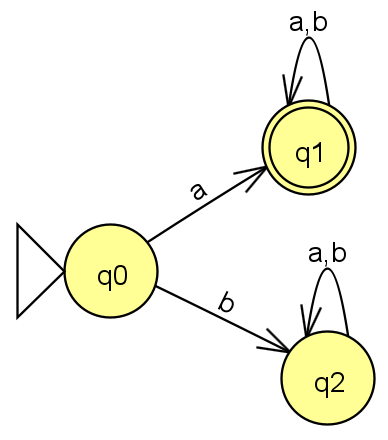
\includegraphics[width=0.2\textwidth]{../../../images/DFAs/ex1_q1.png}\\

2.
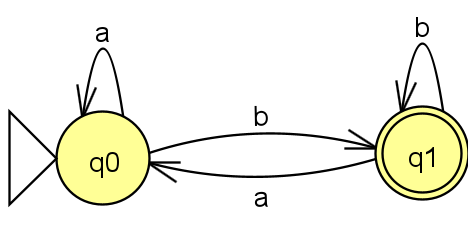
\includegraphics[width=0.2\textwidth]{../../../images/DFAs/ex1_q2.png}\\

3.
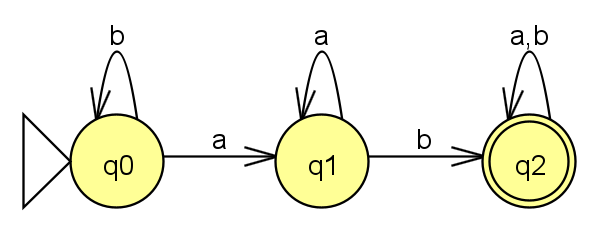
\includegraphics[width=0.3\textwidth]{../../../images/DFAs/ex1_q3.png}\\

4.
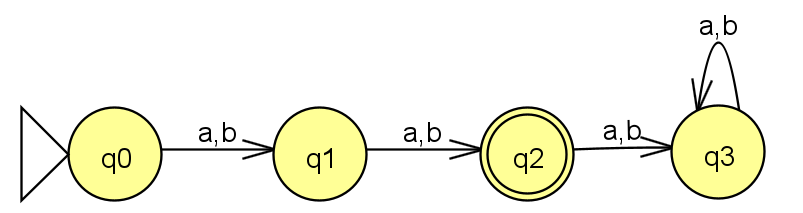
\includegraphics[width=0.4\textwidth]{../../../images/DFAs/ex1_q4.png}\\

5.
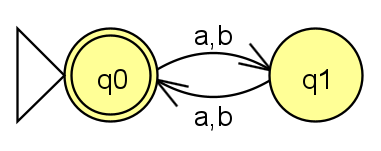
\includegraphics[width=0.2\textwidth]{../../../images/DFAs/ex1_q5.png}\\

6.
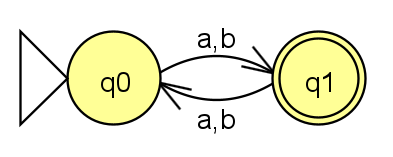
\includegraphics[width=0.2\textwidth]{../../../images/DFAs/ex1_q6.png}\\

7.
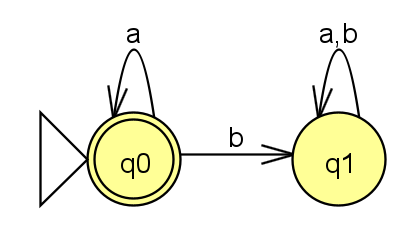
\includegraphics[width=0.2\textwidth]{../../../images/DFAs/ex1_q7.png}\\

8.
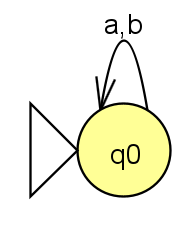
\includegraphics[width=0.1\textwidth]{../../../images/DFAs/ex1_q8.png}\\

9.
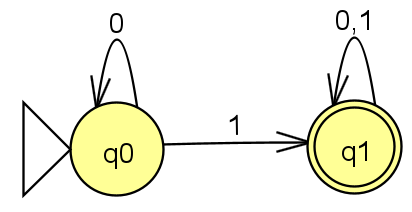
\includegraphics[width=0.2\textwidth]{../../../images/DFAs/ex1_q9.png}\\

10.
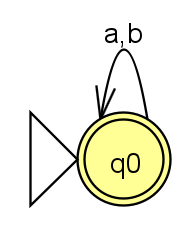
\includegraphics[width=0.1\textwidth]{../../../images/DFAs/ex1_q10.png}

\subsection*{2. بناء أوتومات من اللغة}


لكل لغة من اللغات التالية، ابنِ أوتوماتًا يقبل هذه اللغة.

1.  \textbf{اللغة:} كل السلاسل من الأبجدية $\{0, 1\}$ التي لها عدد زوجي من الأصفار.

2.  \textbf{اللغة:} كل السلاسل من الأبجدية $\{a, b\}$ التي تبدأ وتنتهي بنفس الحرف.

3.  \textbf{اللغة:} كل السلاسل من الأبجدية $\{0, 1\}$ التي طولها يقبل القسمة على 3.

4.  \textbf{اللغة:} كل السلاسل من الأبجدية $\{a, b, c\}$ التي لا تحتوي على السلسلة الفرعية $'ac'$.

5.  \textbf{اللغة:} كل السلاسل من الأبجدية $\{a, b\}$ التي يكون الحرف الثالث من النهاية هو $'a'$.

6.  \textbf{اللغة:} كل السلاسل من الأبجدية $\{0, 1\}$ التي تحتوي على $'1'$ واحدة على الأقل.

7.  \textbf{اللغة:} كل السلاسل من الأبجدية $\{a, b\}$ التي لها عدد فردي من الحرف $'a'$ وعدد فردي من الحرف $'b'$.

8.  \textbf{اللغة:} اللغة التي تحتوي على السلسلة "baba" فقط.

9.  \textbf{اللغة:} كل السلاسل من الأبجدية $\{0, 1\}$ حيث كل $'0'$ تتبعها مباشرة $'1'$.

10. \textbf{اللغة:} كل السلاسل من الأبجدية $\{a, b\}$ التي لا تنتهي بـ $'ab'$.

\end{document}
